\chapter{Polynomials}

\section{Definitions}

\begin{definition}
Let $\mathbb F$ be one of $\Q, \R, \C$ or $\Zm p$ ($p$ prime). A \emph{polynomial} over
$\mathbb F$ is an expression $f(x) = a_nx^n + a_{n-1}x^{n-1} + \cdots + a_1x + a_0$ with
coefficients $a_i \in \mathbb F$. If $a_n \neq 0$, the \emph{degree} is $\deg f = n$ and $a_n$ is
the \emph{leading coefficient}; $f$ is \emph{monic} if $a_n = 1$. The zero polynomial has no
degree. The set of all such polynomials is $\mathbb F[x]$.
\end{definition}

Polynomials are added and multiplied in the usual way. Over a field,
$\deg(fg) = \deg f + \deg g$ for non-zero $f,g$ (Degree of a Product). Two polynomials are
equal iff all corresponding coefficients are equal.

\begin{definition}
$c \in \mathbb F$ is a \emph{root} (zero) of $f$ if $f(c) = 0$. $g$ \emph{divides} $f$,
$g \mid f$, if $f = gh$ for some $h \in \mathbb F[x]$.
\end{definition}

\section{Division algorithm for polynomials}

\begin{theorem}[Division Algorithm for Polynomials, DAP]
Let $f, g \in \mathbb F[x]$ with $g \ne 0$. There exist unique $q, r \in \mathbb F[x]$ with
\[ f = qg + r, \qquad r = 0 \text{ or } \deg r < \deg g. \]
\end{theorem}
\begin{proof}[Proof sketch]
Existence: long division, i.e.\ repeatedly subtract a multiple $\frac{\text{lead}(f)}
{\text{lead}(g)}x^{\deg f - \deg g}g$ of $g$ to kill the leading term; the degree drops each
time (formally, induction on $\deg f$). Uniqueness: if $q_1g + r_1 = q_2g + r_2$ then
$(q_1 - q_2)g = r_2 - r_1$; if $q_1 \ne q_2$ the left side has degree $\ge\deg g$ while the
right has degree $< \deg g$, impossible.
\end{proof}

\begin{example}
Divide $f(x) = 2x^4 + 3x^3 - x + 5$ by $g(x) = x^2 + x - 1$.
\begin{itemize}
  \item $2x^4 / x^2 = 2x^2$; subtract $2x^2 g = 2x^4 + 2x^3 - 2x^2$: remainder so far
        $x^3 + 2x^2 - x + 5$.
  \item $x^3 / x^2 = x$; subtract $xg = x^3 + x^2 - x$: get $x^2 + 5$.
  \item $x^2 / x^2 = 1$; subtract $g = x^2 + x - 1$: get $-x + 6$.
\end{itemize}
So $q(x) = 2x^2 + x + 1$ and $r(x) = -x + 6$. Check:
$(x^2 + x - 1)(2x^2 + x + 1) = 2x^4 + 3x^3 - 1$, and adding $-x + 6$ gives $f$.
\end{example}

\section{Remainder and factor theorems}

\begin{theorem}[Remainder Theorem, RT]
The remainder when $f(x)$ is divided by $x - c$ is $f(c)$.
\end{theorem}
\begin{proof}
By DAP, $f(x) = q(x)(x - c) + r$ with $r$ a constant (degree $< 1$). Substitute $x = c$:
$f(c) = r$.
\end{proof}

\begin{theorem}[Factor Theorem, FT]
$(x - c) \mid f(x)$ if and only if $f(c) = 0$.
\end{theorem}

\begin{example}
The remainder of $f(x) = x^5 + 2x^4 - x^3 + 3x - 7$ upon division by $x + 2$ is
$f(-2) = -32 + 32 + 8 - 6 - 7 = -5$.
\end{example}

\begin{corollary}
A non-zero polynomial of degree $n$ over a field has at most $n$ roots.
\end{corollary}
\begin{proof}
Induction on $n$: if $c$ is a root, $f = (x-c)q$ with $\deg q = n - 1$; any other root $d \ne c$
satisfies $(d - c)q(d) = 0$, so $q(d) = 0$, and $q$ has at most $n - 1$ roots.
\end{proof}

\begin{aside}
This uses that $\mathbb F$ has no zero divisors. In $\Zm 8$, $x^2 - 1$ has four roots
$1,3,5,7$. Compare the four square roots of $4$ mod $35$ in Chapter 9.
\end{aside}

\section{The Fundamental Theorem of Algebra}

\begin{theorem}[Fundamental Theorem of Algebra, FTA]
Every non-constant polynomial in $\C[x]$ has at least one root in $\C$.
\end{theorem}

(The proof requires analysis and is not done in Math 135.) Combined with the factor theorem
and induction on the degree:

\begin{corollary}[Complex Polynomials of Degree $n$ Have $n$ Roots, CPN]
Every $f \in \C[x]$ of degree $n \ge 1$ factors as
\[ f(x) = a_n(x - c_1)(x - c_2)\cdots(x - c_n) \]
with $c_1,\dots,c_n\in\C$ (not necessarily distinct). So $f$ has exactly $n$ roots counted with
multiplicity.
\end{corollary}

The \emph{multiplicity} of a root $c$ is the largest $k$ with $(x - c)^k \mid f$.

\begin{example}
$z^6 - 1 = \prod_{k=0}^{5}(z - \omega^k)$ where $\omega = e^{i\pi/3}$; the roots are the sixth
roots of unity.
\end{example}

\section{Real polynomials: conjugate roots and real factorization}

\begin{theorem}[Conjugate Roots Theorem, CJRT]
If $f \in \R[x]$ and $c\in\C$ is a root of $f$, then $\conj c$ is also a root.
\end{theorem}
\begin{proof}
Since the coefficients are real, $\conj{a_k} = a_k$, so
$f(\conj c) = \sum a_k\conj c^{\,k} = \conj{\sum a_k c^k} = \conj{f(c)} = \conj 0 = 0$ (PCJ).
\end{proof}

For a non-real root $c$, the two factors $x - c$ and $x - \conj c$ combine into a \emph{real}
quadratic:
\[ (x - c)(x - \conj c) = x^2 - 2\RE(c)\,x + \abs c^2. \]

\begin{theorem}[Real Factorization]
Every $f \in \R[x]$ of degree $\ge 1$ can be written as a product of real linear factors and
real quadratic factors with negative discriminant (irreducible over $\R$). In particular, a
real polynomial of odd degree has a real root.
\end{theorem}

\begin{example}
Given that $2i$ is a root of $f(x) = x^4 - 2x^3 + 6x^2 - 8x + 8$, factor $f$ over $\R$ and $\C$.

By CJRT, $-2i$ is also a root, so $(x - 2i)(x + 2i) = x^2 + 4$ divides $f$. Long division:
$f(x) = (x^2 + 4)(x^2 - 2x + 2)$; check: $x^4 - 2x^3 + 2x^2 + 4x^2 - 8x + 8 = f(x)$.
The quadratic $x^2 - 2x + 2$ has discriminant $4 - 8 = -4 < 0$, roots $1 \pm i$. Hence
\begin{align*}
\text{over } \R:&\quad f(x) = (x^2 + 4)(x^2 - 2x + 2),\\
\text{over } \C:&\quad f(x) = (x - 2i)(x + 2i)(x - 1 - i)(x - 1 + i).
\end{align*}
\end{example}

The four roots are placed symmetrically about the real axis, as CJRT requires:
\begin{center}
\begin{tikzpicture}[scale=0.85]
  \draw[->] (-2,0) -- (2.6,0) node[right] {$\RE$};
  \draw[->] (0,-2.6) -- (0,2.7) node[above] {$\IM$};
  \draw[dashed,gray] (-1.8,0) -- (2.4,0);
  \foreach \p/\lab/\pos in {{(0,2)}/{2i}/left,{(0,-2)}/{-2i}/left,{(1,1)}/{1+i}/right,{(1,-1)}/{1-i}/right} {
    \fill[red!70!black] \p circle (2.5pt) node[\pos,font=\small] {$\lab$};
  }
  \draw[<->,gray] (0.15,1.75) -- (0.15,-1.75);
  \draw[<->,gray] (1,0.75) -- (1,-0.75);
  \node[font=\scriptsize,gray,align=center] at (-1.3,1.1) {conjugate\\pairs};
\end{tikzpicture}
\end{center}

\begin{example}
Factor $x^6 - 1$ over $\R$. Its roots are the sixth roots of unity
$\pm 1$, $\frac12\pm\frac{\sqrt3}2 i$, $-\frac12 \pm \frac{\sqrt3}2 i$. Pairing conjugates
($\RE = \pm\frac12$, $\abs{c}^2 = 1$):
\[ x^6 - 1 = (x - 1)(x + 1)(x^2 - x + 1)(x^2 + x + 1). \]
\end{example}

\begin{important}[CJRT needs real coefficients]
$f(z) = z - i$ has root $i$ but not $-i$. The theorem fails for polynomials with non-real
coefficients.
\end{important}

\section{Rational roots}

\begin{theorem}[Rational Roots Theorem, RRT]
Let $f(x) = a_nx^n + \cdots + a_0 \in \Z[x]$ with $a_n \ne 0$. If $\frac pq$ is a root in lowest
terms ($\gcd(p,q) = 1$, $q > 0$), then $p \mid a_0$ and $q \mid a_n$.
\end{theorem}
\begin{proof}
Multiply $f(p/q) = 0$ by $q^n$:
$a_np^n + a_{n-1}p^{n-1}q + \cdots + a_1pq^{n-1} + a_0q^n = 0$. Every term except $a_0q^n$ is a
multiple of $p$, so $p \mid a_0q^n$; as $\gcd(p,q^n) = 1$, CAD gives $p \mid a_0$. Similarly every
term except $a_np^n$ is a multiple of $q$, so $q \mid a_n$.
\end{proof}

\begin{example}
Factor $f(x) = 2x^3 + x^2 - 7x - 6$ over $\Q$.
Candidates $p/q$ with $p \mid 6$, $q \mid 2$: $\pm1, \pm2, \pm3,\pm6,\pm\frac12,\pm\frac32$.
Try $x = -1$: $-2 + 1 + 7 - 6 = 0$. So $(x + 1) \mid f$, and division gives
$f(x) = (x+1)(2x^2 - x - 6)$. Factoring the quadratic, $2x^2 - x - 6 = (2x + 3)(x - 2)$, so
\[ f(x) = (x + 1)(2x + 3)(x - 2), \]
with roots $-1, -\frac32, 2$, all among the candidates.
\end{example}

\begin{center}
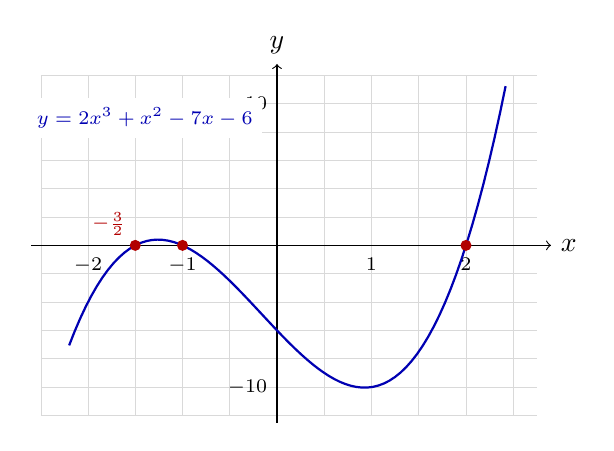
\begin{tikzpicture}[x=1.2cm,y=0.18cm]
  \draw[very thin,gray!30] (-2.5,-12) grid[xstep=0.5,ystep=2] (2.75,12);
  \draw[->] (-2.6,0) -- (2.9,0) node[right] {$x$};
  \draw[->] (0,-12.5) -- (0,12.8) node[above] {$y$};
  \foreach \x in {-2,-1,1,2} { \node[below,font=\scriptsize] at (\x,-0.2) {$\x$}; }
  \foreach \y in {-10,10} { \node[left,font=\scriptsize] at (0,\y) {$\y$}; }
  \draw[thick,blue!70!black,domain=-2.2:2.42,samples=80] plot (\x,{2*(\x)^3+(\x)^2-7*\x-6});
  \foreach \r in {-1.5,-1,2} { \fill[red!70!black] (\r,0) circle (2pt); }
  \node[font=\scriptsize,red!70!black,above left] at (-1.5,0) {$-\frac32$};
  \node[font=\scriptsize,blue!70!black,fill=white] at (-1.4,9) {$y = 2x^3 + x^2 - 7x - 6$};
\end{tikzpicture}
\end{center}

\begin{example}
$x^3 - 3x - 1$ has no rational roots: the only candidates are $\pm1$, and $f(1) = -3$,
$f(-1) = 1$. Since a cubic that factors over $\Q$ must have a linear factor, $x^3 - 3x - 1$ is
irreducible over $\Q$. (It still has three real roots, by the intermediate value theorem.)
\end{example}

\begin{center}
\begin{tikzpicture}[x=1.3cm,y=0.45cm]
  \draw[->] (-2.4,0) -- (2.5,0) node[right] {$x$};
  \draw[->] (0,-4.5) -- (0,4.5) node[above] {$y$};
  \draw[thick,blue!70!black,domain=-2.2:2.15,samples=80] plot (\x,{(\x)^3-3*\x-1});
  \foreach \x/\v in {-2/-3,-1/1,0/-1,1/-3,2/1} {
    \fill (\x,\v) circle (1.5pt);
    \node[font=\scriptsize,below] at (\x,-4.6) {$\x$};
  }
  \foreach \r in {-1.532,-0.347,1.879} { \fill[red!70!black] (\r,0) circle (2pt); }
  \node[font=\scriptsize,blue!70!black,right] at (1.25,3.3) {$y = x^3 - 3x - 1$};
\end{tikzpicture}
\end{center}
The values at $x = -2,-1,0,1,2$ are $-3, 1, -1, -3, 1$; the three sign changes trap the
three real roots (red), none of which is rational.

\section{Polynomials over $\Zm p$}

The division algorithm and factor theorem work over $\Zm p$ as well. For example, over $\Zm 5$,
$x^2 + 1$ has roots $2$ and $3$ ($4 + 1 = 5 \equiv 0$, $9 + 1 = 10 \equiv 0$), so
$x^2 + 1 = (x - 2)(x - 3) = (x + 3)(x + 2)$ in $\Zm 5[x]$, while over $\Zm 3$ it has no roots
($0^2+1=1$, $1^2+1 = 2$, $2^2+1 = 5 \equiv 2$) and is irreducible. By FLT, $x^p - x =
\prod_{a\in\Zm p}(x - a)$ in $\Zm p[x]$.

\section{Common pitfalls}
\begin{itemize}
  \item Forgetting zero coefficients when doing long division (write $2x^4 + 3x^3 + 0x^2 - x
        + 5$).
  \item Applying CJRT to a polynomial with complex coefficients.
  \item Applying RRT to non-integer coefficients (clear denominators first) or forgetting
        negative candidates.
  \item Stopping at ``irreducible over $\R$'' when the question asks for a factorization over
        $\C$.
\end{itemize}

\section{Summary}
\begin{itemize}
  \item DAP: $f = qg + r$ with $\deg r < \deg g$. RT: $f(c)$ is the remainder mod $x - c$;
        FT: $f(c) = 0 \iff (x - c)\mid f$.
  \item FTA: every non-constant complex polynomial has a root; degree $n$ means exactly $n$
        roots with multiplicity.
  \item CJRT: real polynomials have non-real roots in conjugate pairs; real polynomials factor
        into real linear and irreducible quadratic factors.
  \item RRT: rational roots $p/q$ of integer polynomials have $p \mid a_0$, $q \mid a_n$.
\end{itemize}
